



\begin{figure}[b]
  \centering
  \begin{subfigure}[b]{0.45\linewidth}
    \centering
    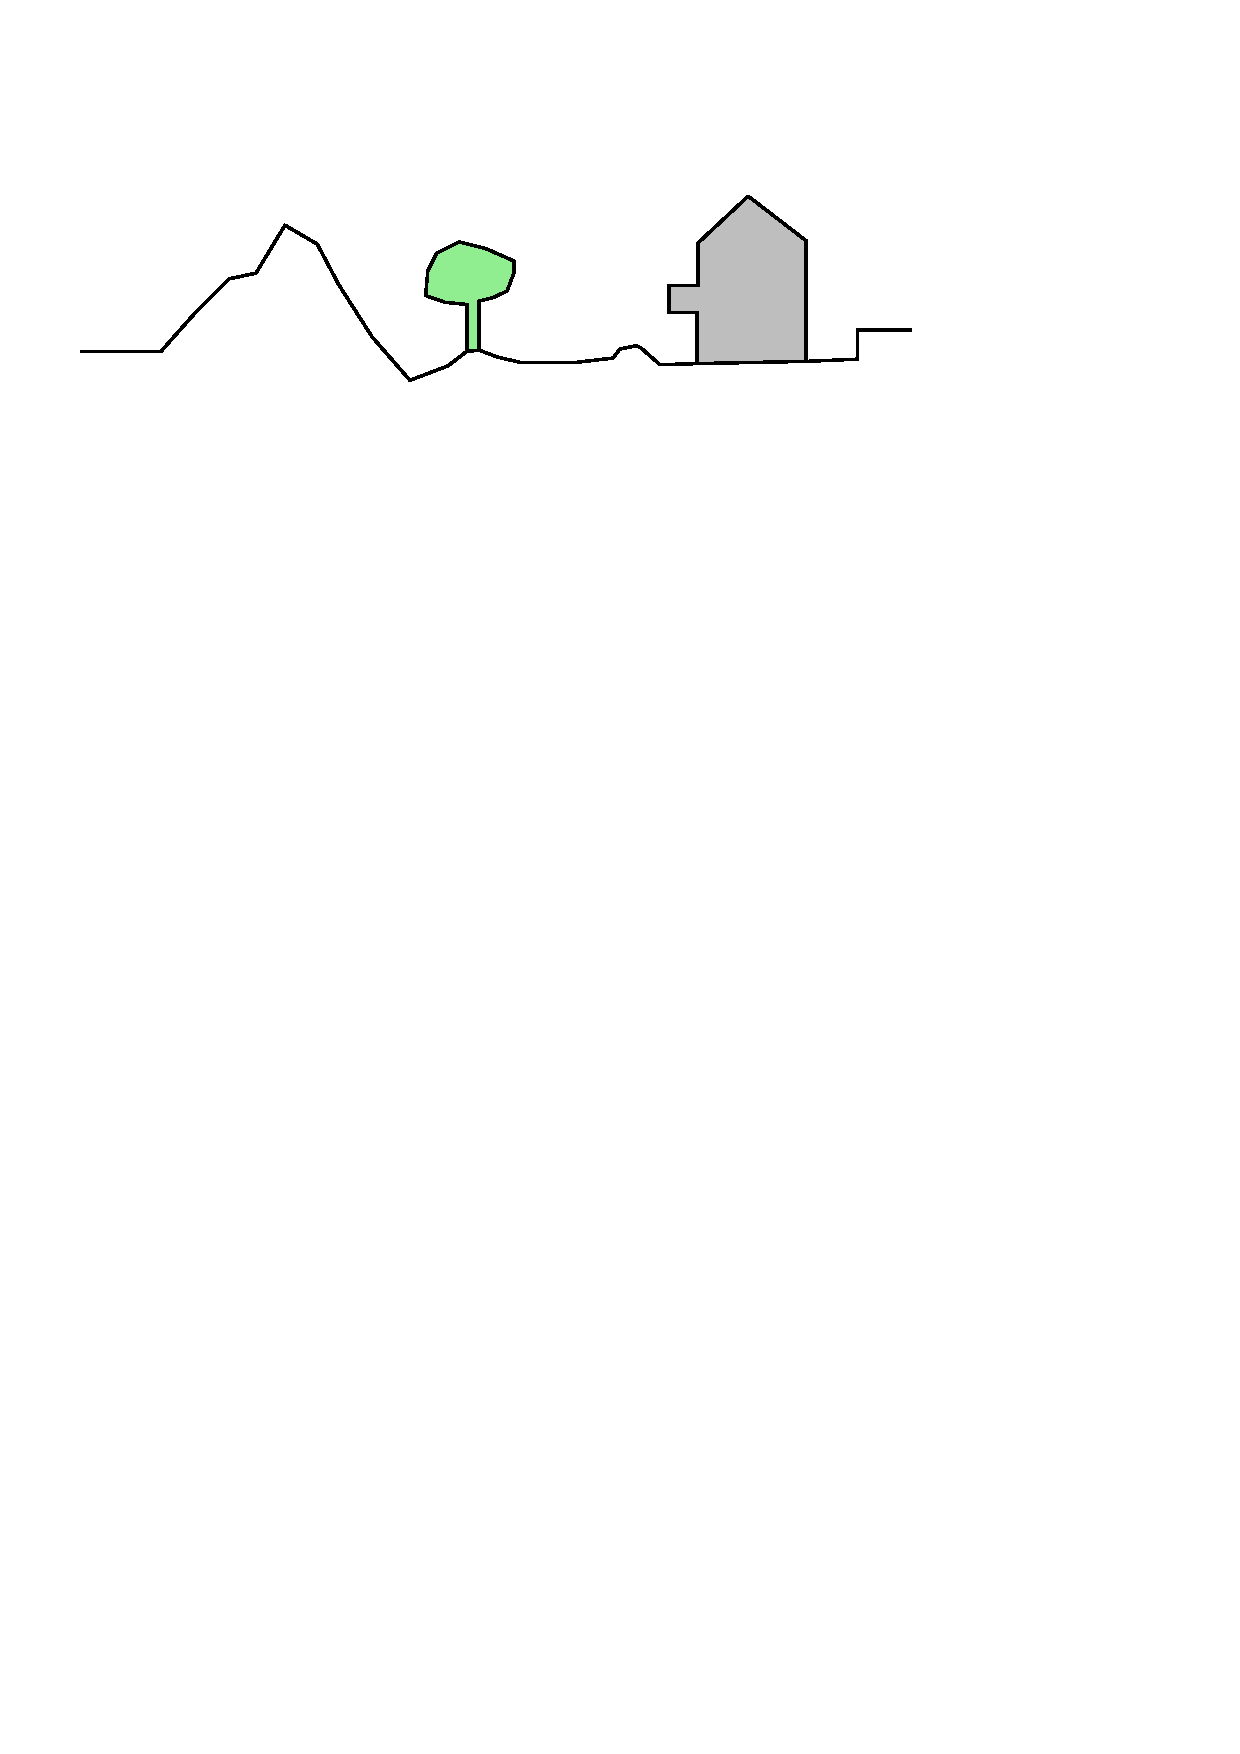
\includegraphics[page=1,width=\linewidth]{figs/dimgis}
    \caption{A terrain}\label{fig:dimgis:1}
  \end{subfigure}%
  \qquad %-- that adds some space between th 2 figures
  \begin{subfigure}[b]{0.45\linewidth}
    \centering
    \includegraphics[page=6,width=\linewidth]{figs/dimgis}
    \caption{2.5D modelling}\label{fig:dimgis:25}
  \end{subfigure}%
  \qquad %-- that adds some space between th 2 figures
  \begin{subfigure}[b]{0.45\linewidth}
    \centering
    \includegraphics[page=5,width=\linewidth]{figs/dimgis}
    \caption{2.75D modelling}\label{fig:dimgis:275}
  \end{subfigure}%
  \qquad %-- that adds some space between th 2 figures
  \begin{subfigure}[b]{0.45\linewidth}
    \centering
    \includegraphics[page=4,width=\linewidth]{figs/dimgis}
    \caption{Volumetric modelling, or full 3D}\label{fig:dimgis:3}
  \end{subfigure}%
  \caption{Different meanings for `3D GIS' in the context of terrains.}
\label{fig:dimgis}
\end{figure}













\begin{figure}
	\centering
	\begin{subfigure}{0.4\linewidth}
		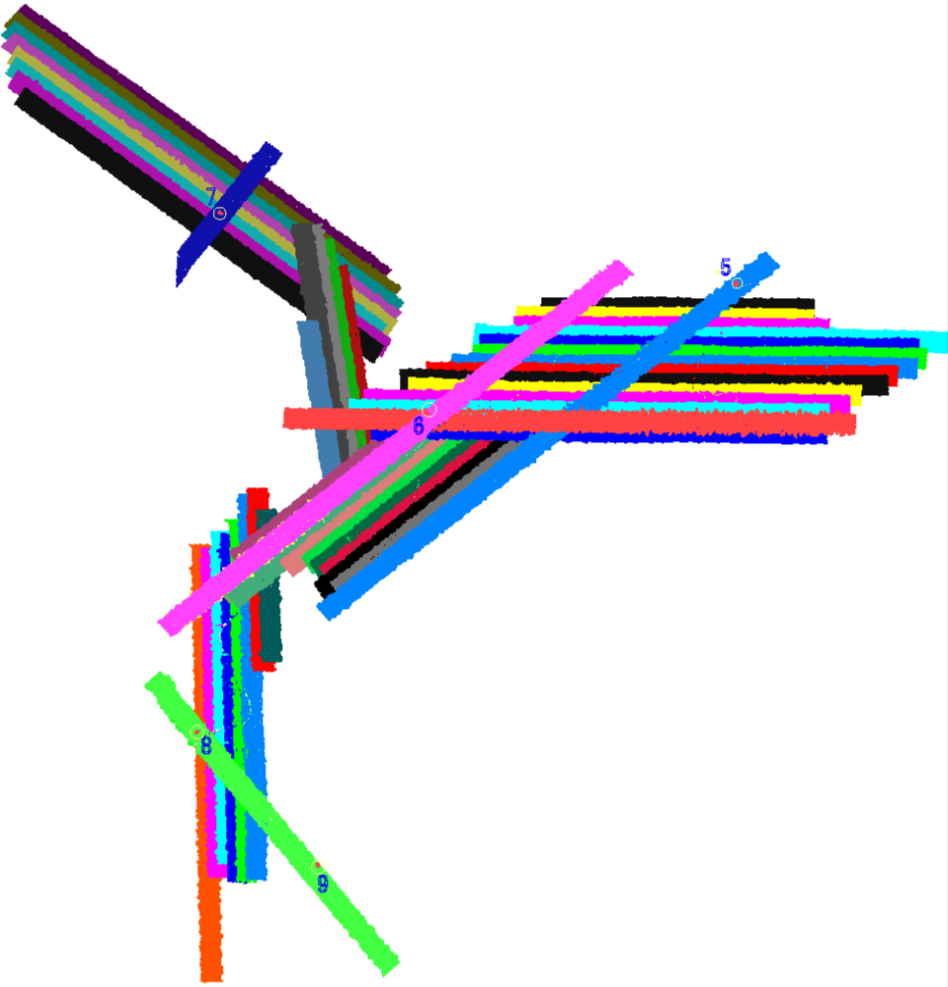
\includegraphics[width=\textwidth]{figs/lidar_strips.png}
		\subcaption{Plan view of the different strips of a lidar survey \citep{Kornus03}}
		\label{fig:lidarStrips}
	\end{subfigure}
	\quad
	\begin{subfigure}{0.4\linewidth}
		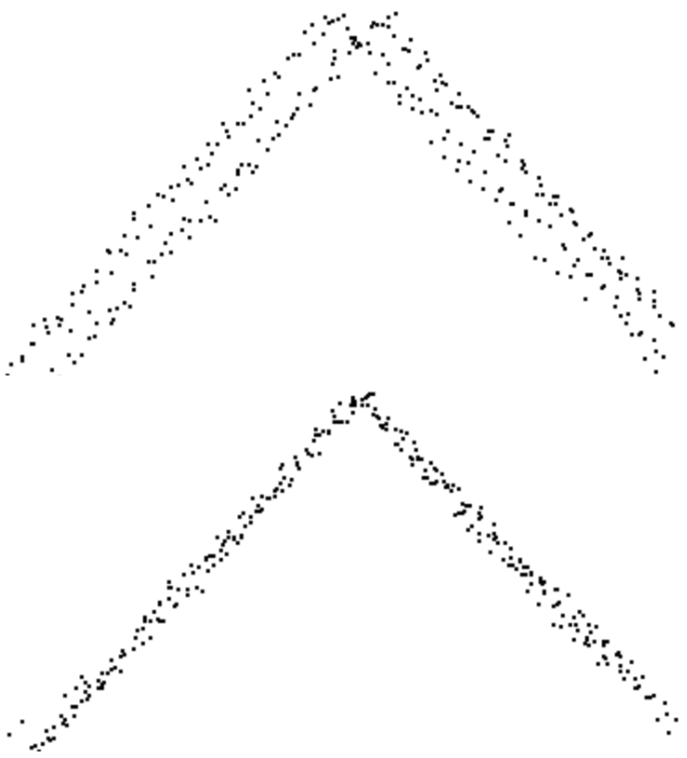
\includegraphics[width=\textwidth]{figs/strip_adjustment.png}
		\subcaption{Cross-section of gable roof before (top) and after (bottom) strip adjustment \citep{Vosselman02}}
		\label{fig:lidarGableRoof}
	\end{subfigure}
	\caption{Strip adjustment for lidar point clouds}
	\label{fig:lidarStripAdj}
\end{figure}